%This work is licensed under the Creative Commons License Attribution 4.0 International (CC-BY 4.0)
%https://creativecommons.org/licenses/by/4.0/legalcode
\documentclass[rgb]{standalone}
\usepackage{pgfplots}
\usepgfplotslibrary{patchplots}
\pgfplotsset{colormap/viridis}
\begin{document}
	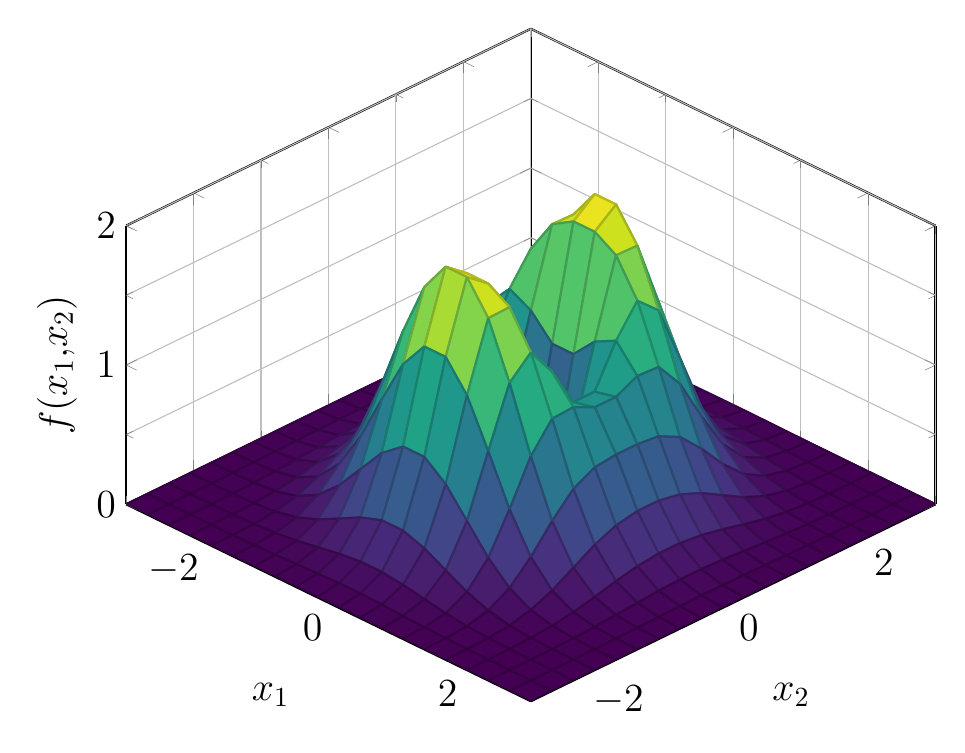
\begin{tikzpicture}[font=\Large]
		\begin{axis}[scale=1.5,thick,grid=both, minor tick num =1,view={45}{45},
			xmin=-3, xmax=3, ymin=-3,ymax=3, zmin=0, zmax=2, 
			ztick={0,1,2}, 
			xlabel=$x_1$, ylabel=$x_2$, zlabel=$f(x_1 {,} x_2)$]
		\addplot3[surf, patch, domain=-3:3, y domain=-3:3,
			samples=20] {(x^2+2*y^2)*exp(1-x^2-y^2)};
		\end{axis}
	\end{tikzpicture}
\end{document}